\documentclass{article}
\usepackage[utf8]{inputenc}
\usepackage{graphicx}
\usepackage{caption}
\usepackage{hyperref}
\usepackage{tcolorbox}
\tcbuselibrary{theorems}


\newtcbtheorem[no counter]{need}{Need}%
{ 
  sharp corners,
  colback=green!5,
  colframe=green!25,
  fonttitle=\bfseries,
  coltitle=black,
 }{th}

\begin{document}

\begin{center}

\includegraphics[width=\textwidth]{data/logocircle.png}
\title{Relazione greenLivery}
\author{Flavio, Nicola, Luca, Matteo, Mario}
\end{center}
\renewcommand{\contentsname}{Indice}

\maketitle
\tableofcontents

\section{Inizio del progetto}\par

Il topic del progetto dato dal professore, è la realizzazione di un servizio legato a cibo e alimentazione. Con particolare aree di interessi,come: \par
\begin{itemize}
    \item \textbf{dieta}:gestione dieta per uno stile di vita sano, e.g., per motivi medici/altro, dieta per sportivi, gestione ricettari, diario della dieta \par
    \item \textbf{green}:cambiamento abitudini alimentari, diminuzione di food-waste e risorse impiegate (e.g., per produrre carne), gestione smart di coltivazioni e allevamenti \par
    \item \textbf{cultura}: tradizioni alimentari, prodotti tipici del territorio, percorsi enogastronomici, slowfood\par
    \item \textbf{aggregazione/commercio}: ristoranti, bar, delivery della spesa o di piatti pronti \par
    \item \textbf{tecnologia}: tele-dining (e.g., aperitivo da remoto), mukbang (guardare altri mangiare su YouTube), food printing, ... \par
\end{itemize}
\vspace{1cm}



    \addcontentsline{toc}{subsection}{\numberline{1.1}Argomento del nostro progetto} \par
    \numberline{\fontsize{4mm}{1mm}\selectfont \textbf{1.1 Argomento del nostro progetto}}
    Il nostro scopo è quello di sviluppare un’applicazione di food delivery completamente Green, data l'elevata criticità raggiunta negli ultimi periodi soprattutto a causa dell'eccessivo aumento delle temperature. Visto che una delle principali cause è dovuta alle alte emissioni di CO2, anche se potrebbe non essere una soluzione finale, utilizzare veicoli elettrici al posto di veicoli termici, aiuta l’ambiente permettendo comunque di avere le stesse tempistiche e la stessa qualità di consegna.
    \vspace{1cm}
    
    \addcontentsline{toc}{subsection}{\numberline{1.2}Analisi app competitor} \par
    \numberline{\fontsize{4mm}{1mm}\selectfont\textbf{1.2 Confronto con app simili}}
    Analizzando le principali app di food delivery è emerso che: tutte posseggono sia un sito web che un'app per smartphone, ci permettono di geolocalizzare il nostro indirizzo e ci consigliano iristoranti.
    Abbiamo individuato le seguenti app competitor:
\begin{itemize}
        \item \textbf{App n1 - \href{https://www.justeat.it}{JustEat}:} Ha un’interfaccia intuitiva, con le categorie e la ricerca in primo piano, non permette però di visualizzare il nome e la foto del rider. Non è neanche possibile chattare con il rider e il ristorante.

        \item \textbf{App n2 - \href{https://glovoapp.com/it/it/}{Glovo}:} Interfaccia divisa in macrocategorie che ci offre servizi diversi dalla concorrenza, come inviare pacchi da un indirizzo all’altro o ordinare farmaci. É possibile visualizzare delle informazione sul rider come la posizione in tempo reale e chattare con lui. Offre anche la possibilità di accumulare credito sull’app invitando degli amici ad iscriversi. É possibile inoltre recensire il ristorante, l’ordine ricevuto e il rider che lo ha consegnato.

        \item \textbf{App n3 - \href{https://deliveroo.it/it/}{Deliveroo}:} Come JustEat ci offre in homepage le varie categorie, le promozioni in corso e la ricerca dei ristoranti. Ci permette di visualizzare info e posizione del rider ed è possibile recensire ristorante, ordine e rider come Glovo. La peculiarità di questa app è poter aggiungere alcuni ristoranti tra i preferiti e visualizzarli facilmente tramite un pulsante in homepage. Aprendo le categorie è possibile filtrare i ristoranti in base a regimi alimentari (Vegano, senza glutine, kosher ...).

        \item \textbf{App n4 - \href{https://www.ubereats.com/it/}{UberEats}:} Schermata intuitiva ma con meno categorie presenti rispetto ai competitor. Offre la possibilità di visualizzare tutte le info e la posizione del rider e ci permette inoltre di recensire non solo il ristorante e il rider, ma anche singolarmente ogni prodotto dell’ordine che abbiamo fatto.

\end{itemize}
Abbiamo la conferma delle app competitor conosciute da parte degli utenti che hanno risposto al nostro form, nel seguente modo:
\begin{center}
   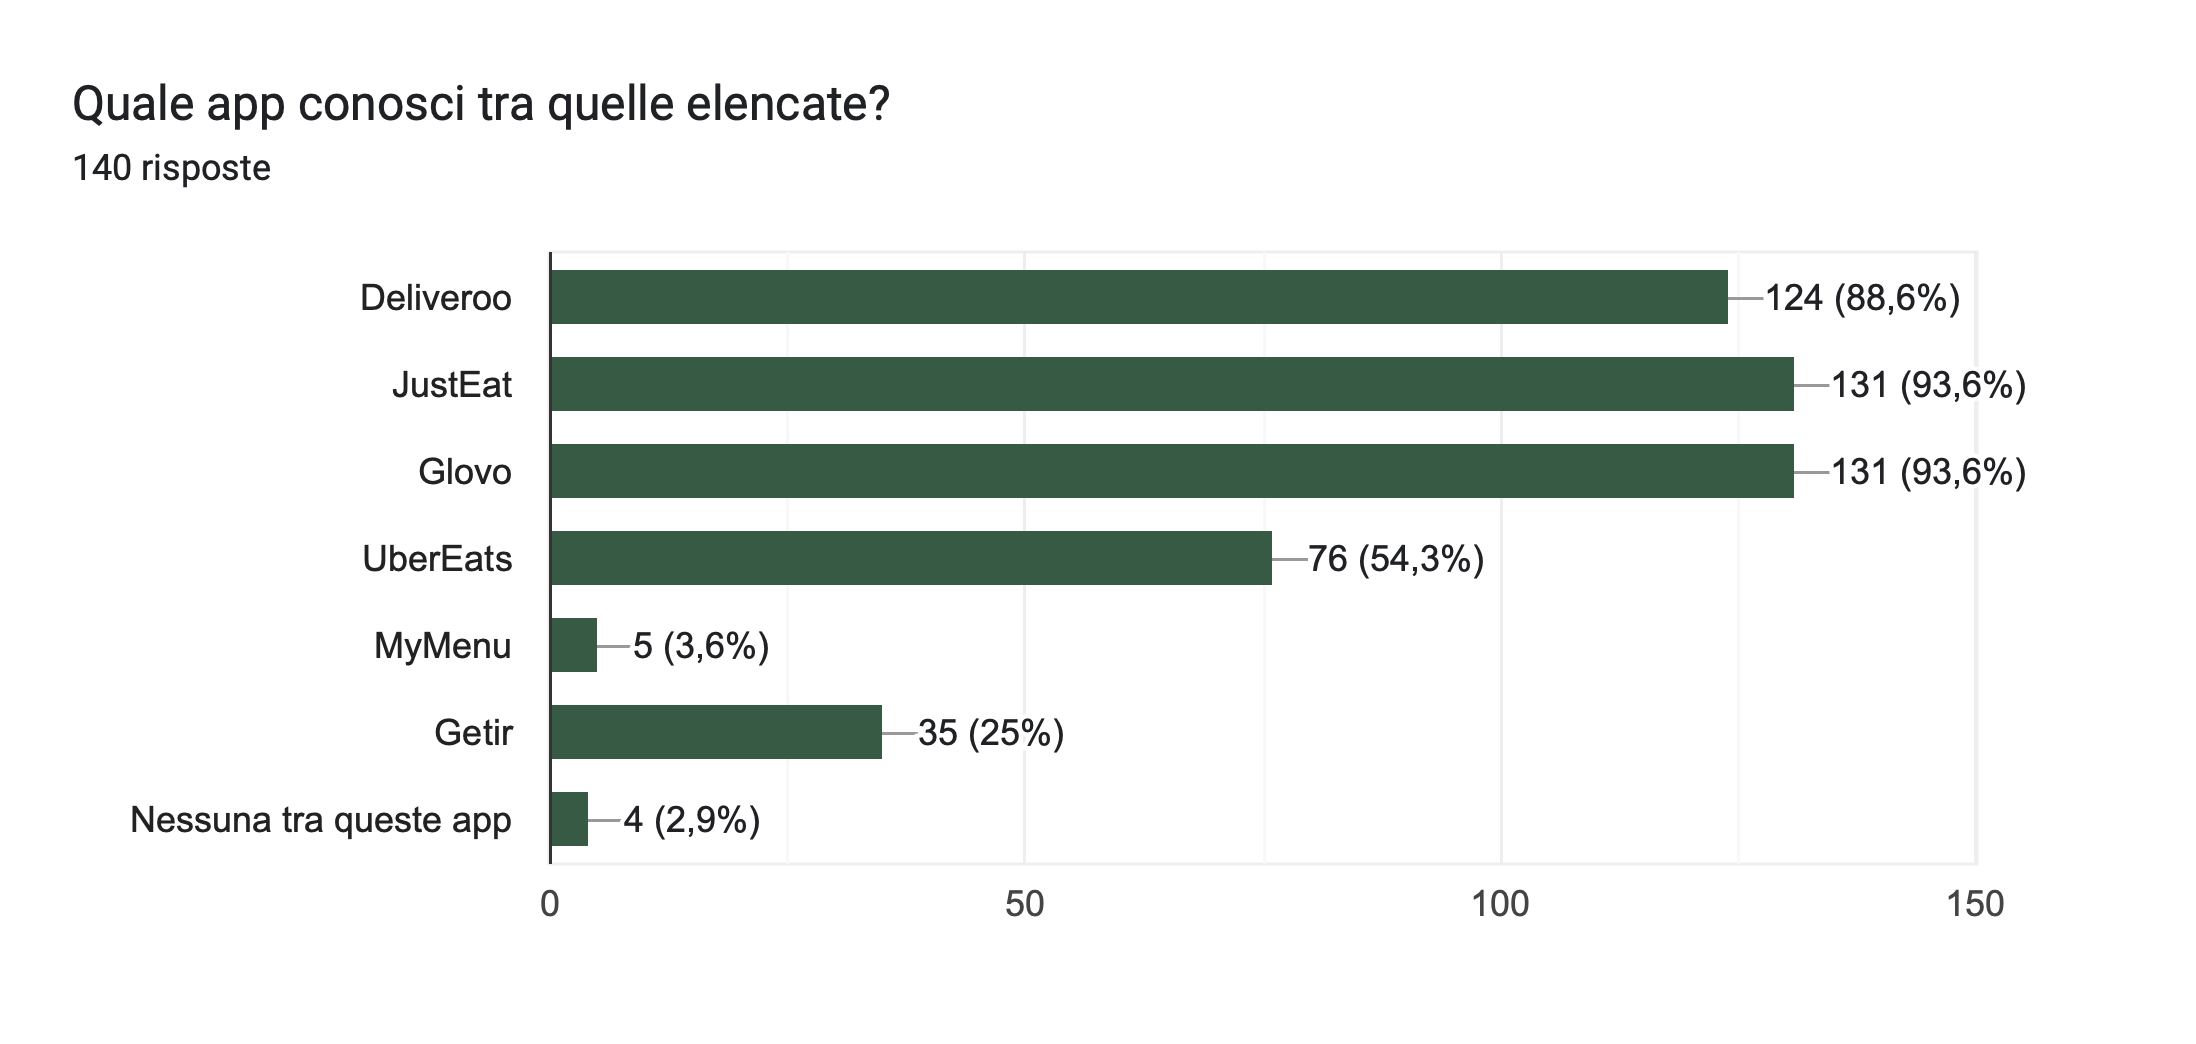
\includegraphics[width=\textwidth]{App_competitor.png} 
\end{center}
\par In seguito ne abbiamo avuto la conferma:
\begin{center}
    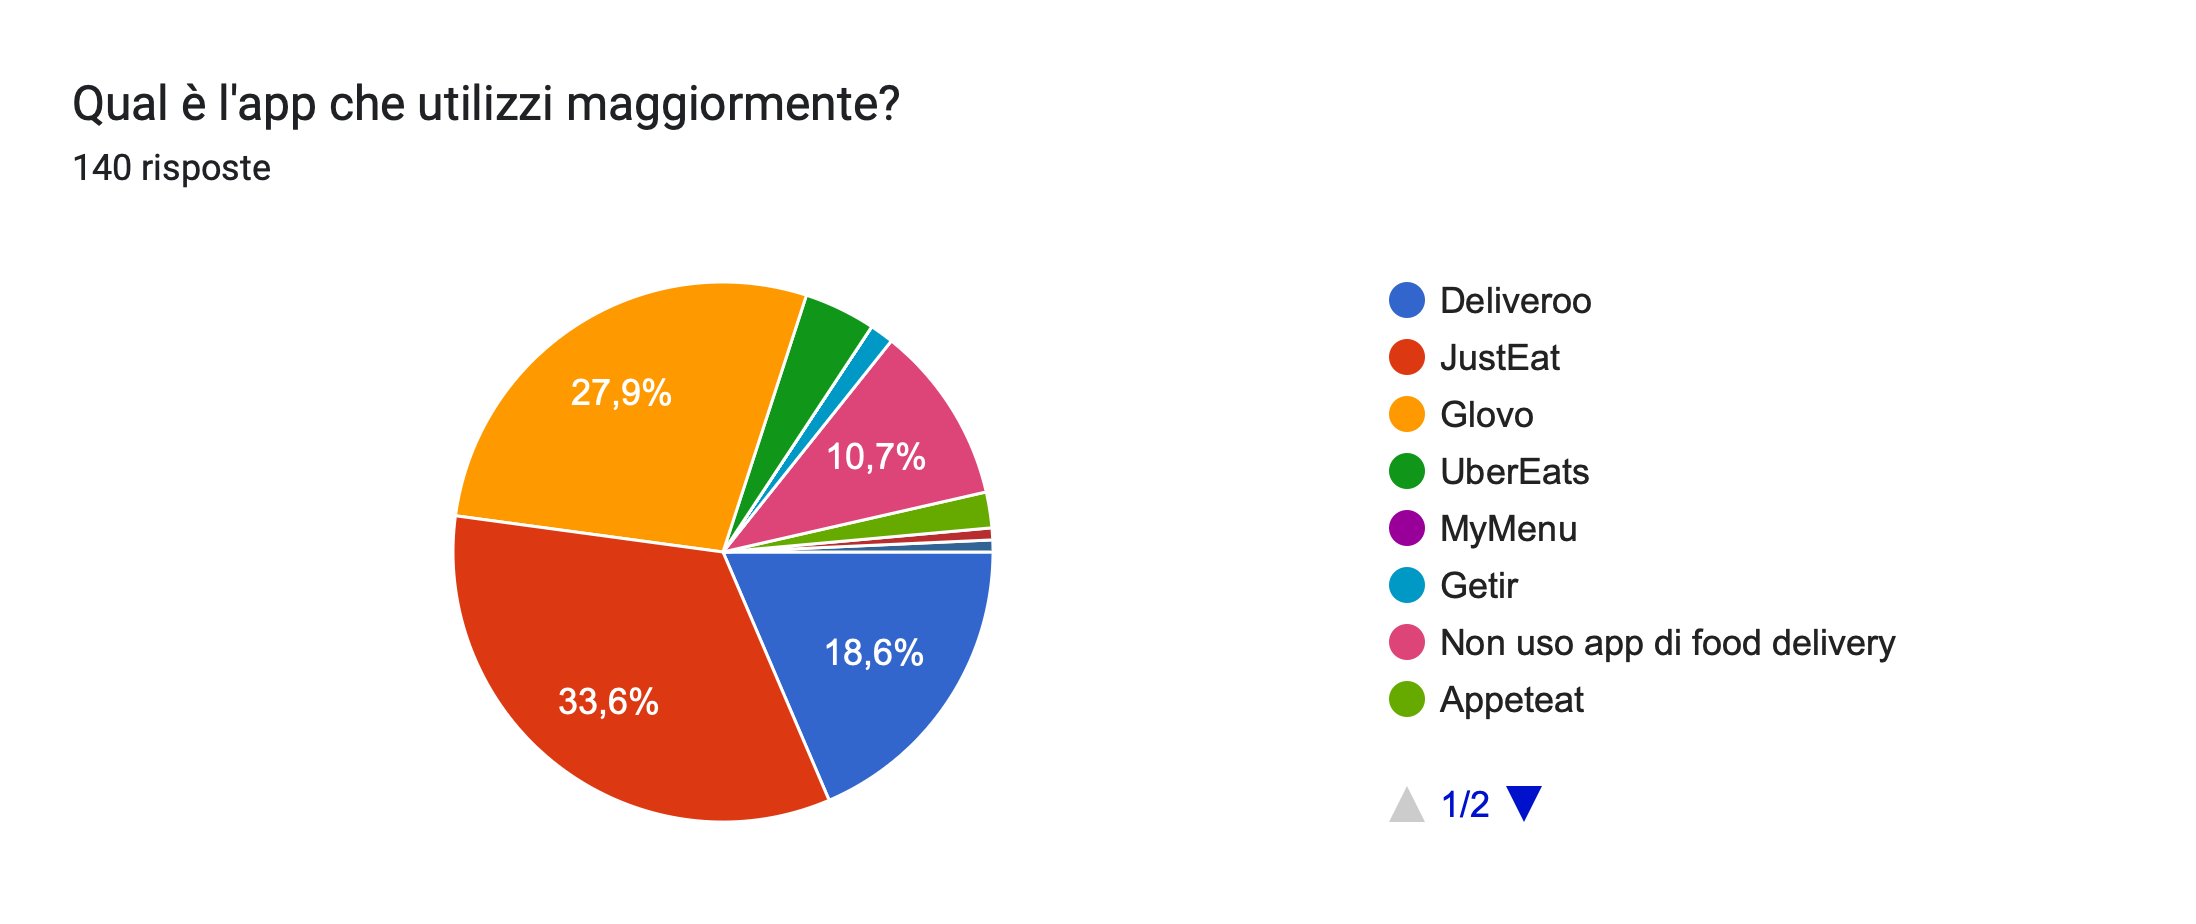
\includegraphics[width=\textwidth]{App_competitor_utilizzate.png}
\end{center}


    \vspace{1cm}
\section{Needfinding} 
In questa fase di sviluppo l’obiettivo è comprendere le necessità degli utenti nella capire perchè è meglio utilizzare un'app.
    \vspace{1cm}
    \addcontentsline{toc}{subsection}{\numberline{2.1}Interviste} \par
    \numberline{\fontsize{4mm}{1mm}\selectfont \textbf{2.1 Interviste}}
\par Per le interviste abbiamo realizzato due versioni, composte rispettivamente da 5 e 6 domande, utilizzando la prima versione come pilota e con l'aiuto della versione 1 siamo riusciti a fare delle domande più complete. \par Le interviste sono state poste per lo più, a colleghi di università, amici, e colleghi di lavoro, per una durata media di 10 minuti.\par
  \vspace{1cm}
\addcontentsline{toc}{subsubsection}{\numberline{2.1.1}Domande}\par\numberline{\fontsize{4mm}{1mm}\selectfont \textbf{2.1.1 Domande}}
    \begin{enumerate}
    
     \item \textit{Ordini mai a domicilio?}
        \begin{enumerate}
            \item Se no, perchè?
        \end{enumerate}
     \item \textit{Conoscete e avete mai utilizzato un'app di food delivery?}
     \begin{enumerate}
         \item Quali?
         \item Quanto spesso le usi?
     \end{enumerate}
     \item \textit{Quali funzionalità preferisci dell'app che utilizzi?}
     \item \textit{Quali potrebbero essere delle funzionalità che ti potrebbero tornare utilizi ma che non sono implementate?}
    \item \textit{Ti farebbe comodo conoscere i valori nutrizionali(calorie, proteine, carboidrati, grassi) delle pietanze che ordini?}
    \begin{enumerate}
        \item La troveresti utile se dovessi seguire una dieta?
    \end{enumerate}
    \item \textit{Vista l'attuale situazione climatica globale, favoriresti un servizio di cosegna a domicilio completamente Green? Se si, perchè? }
    \begin{enumerate}
        \item Anche se questo dovesse comportare dei costi leggermente maggiori?
    \end{enumerate}
\end{enumerate}

    \vspace{1cm}
 
    \addcontentsline{toc}{subsection}{\numberline{2.2}Questionari} \par 
    \numberline{\fontsize{4mm}{1mm}\selectfont \textbf{2.2 \href{https://forms.gle/LbzJgv2mBttKMyoz5}{Questionari}}}
\par E' stato condotto un questionario che permette di raggiungere un numero di partecipanti decisamente maggiore,per confermare se i need individuati con le interviste sono corretti.\par Inoltre permette di visualizzare in modo più preciso le preferenze degli utenti tramite grafici significativi:
\par \vspace{1cm}
Sono state ottenute \textbf{158} risposte che andremo ad analizzare con l'aiuto dei grafici significati ottenuti su Google Moduli.\par 
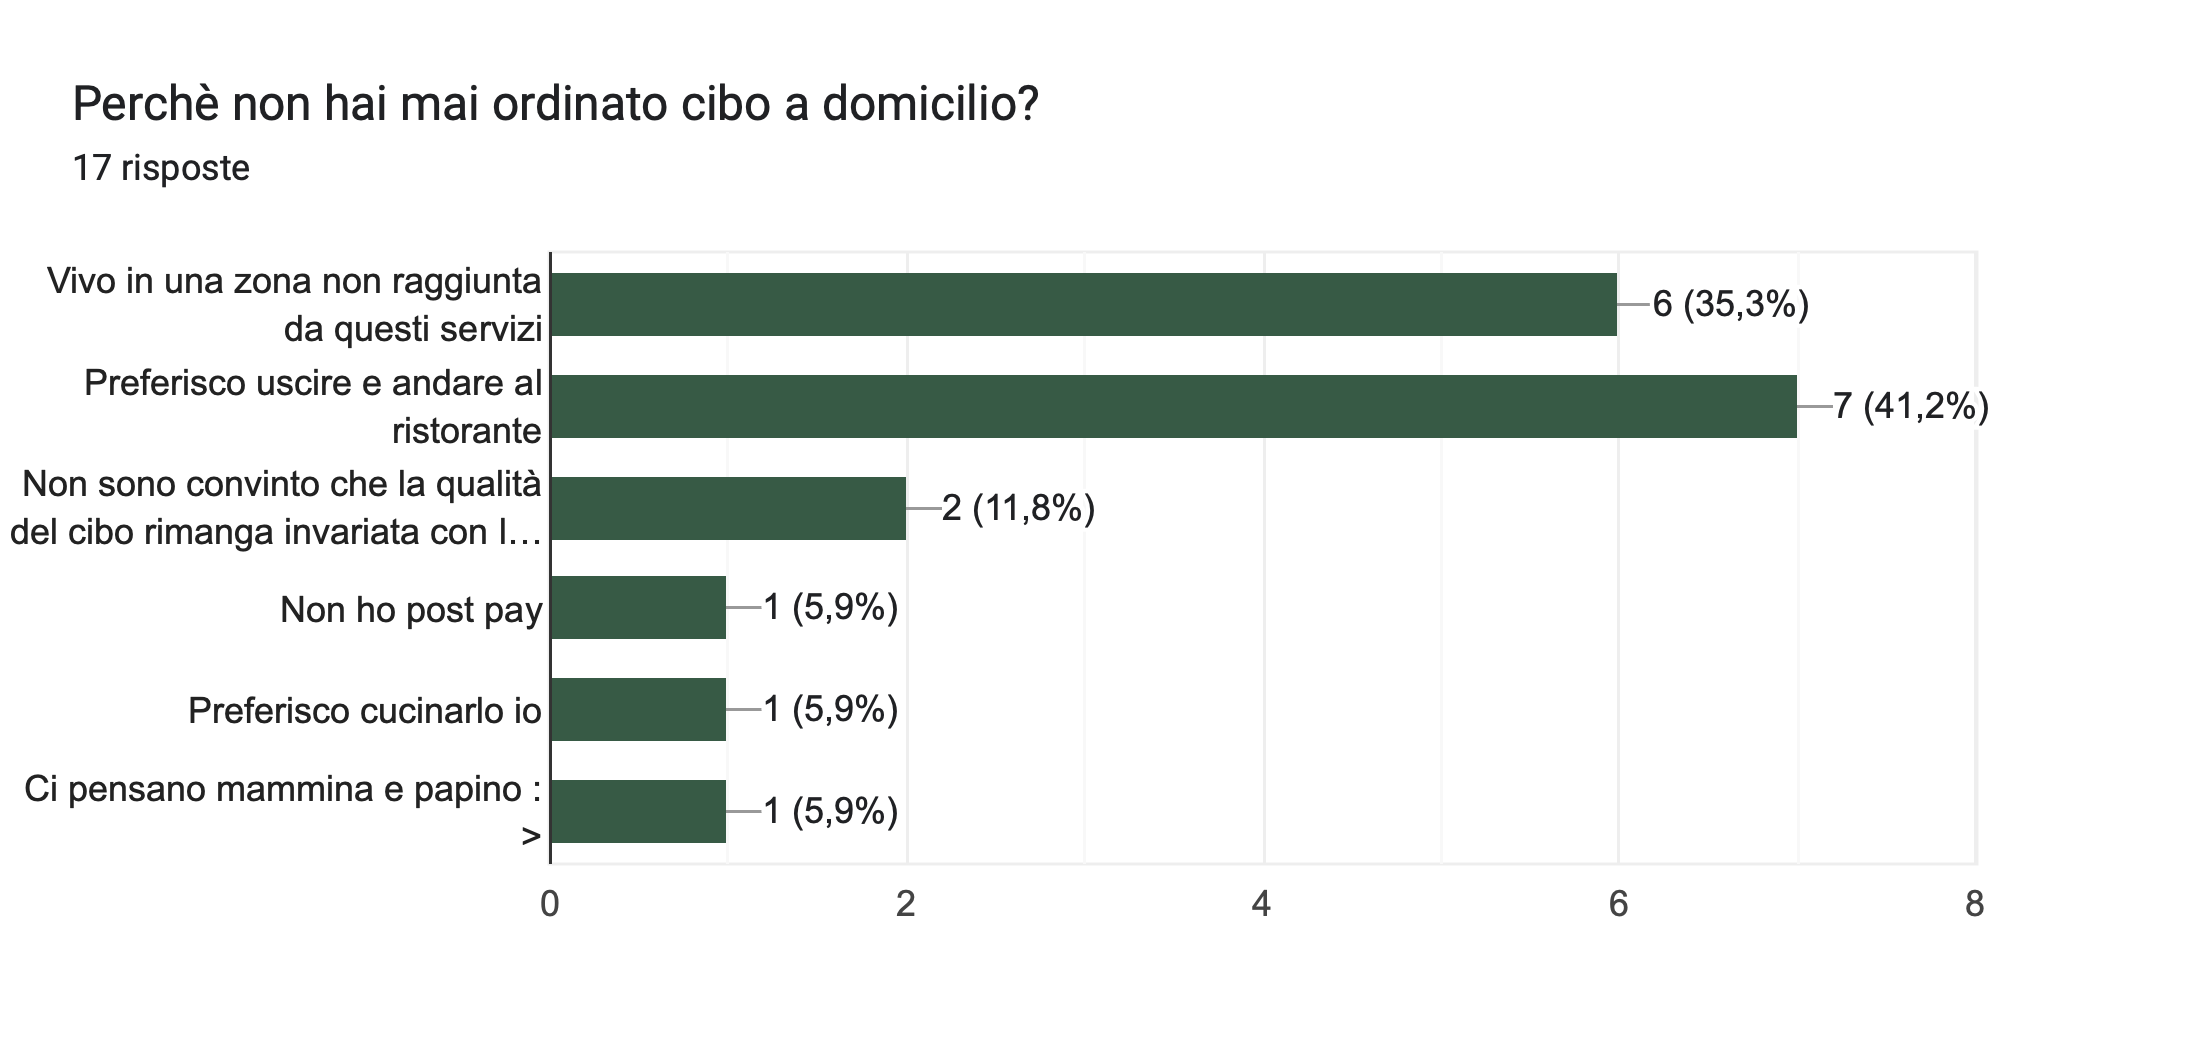
\includegraphics[width=\textwidth]{Perche_non_ordina.png}
Come tematica non da sottovalutare, e il \textbf{perchè} molti utenti non utilizzano un servizio dedicato per le consegne a domicilio.\vspace{1cm}\par
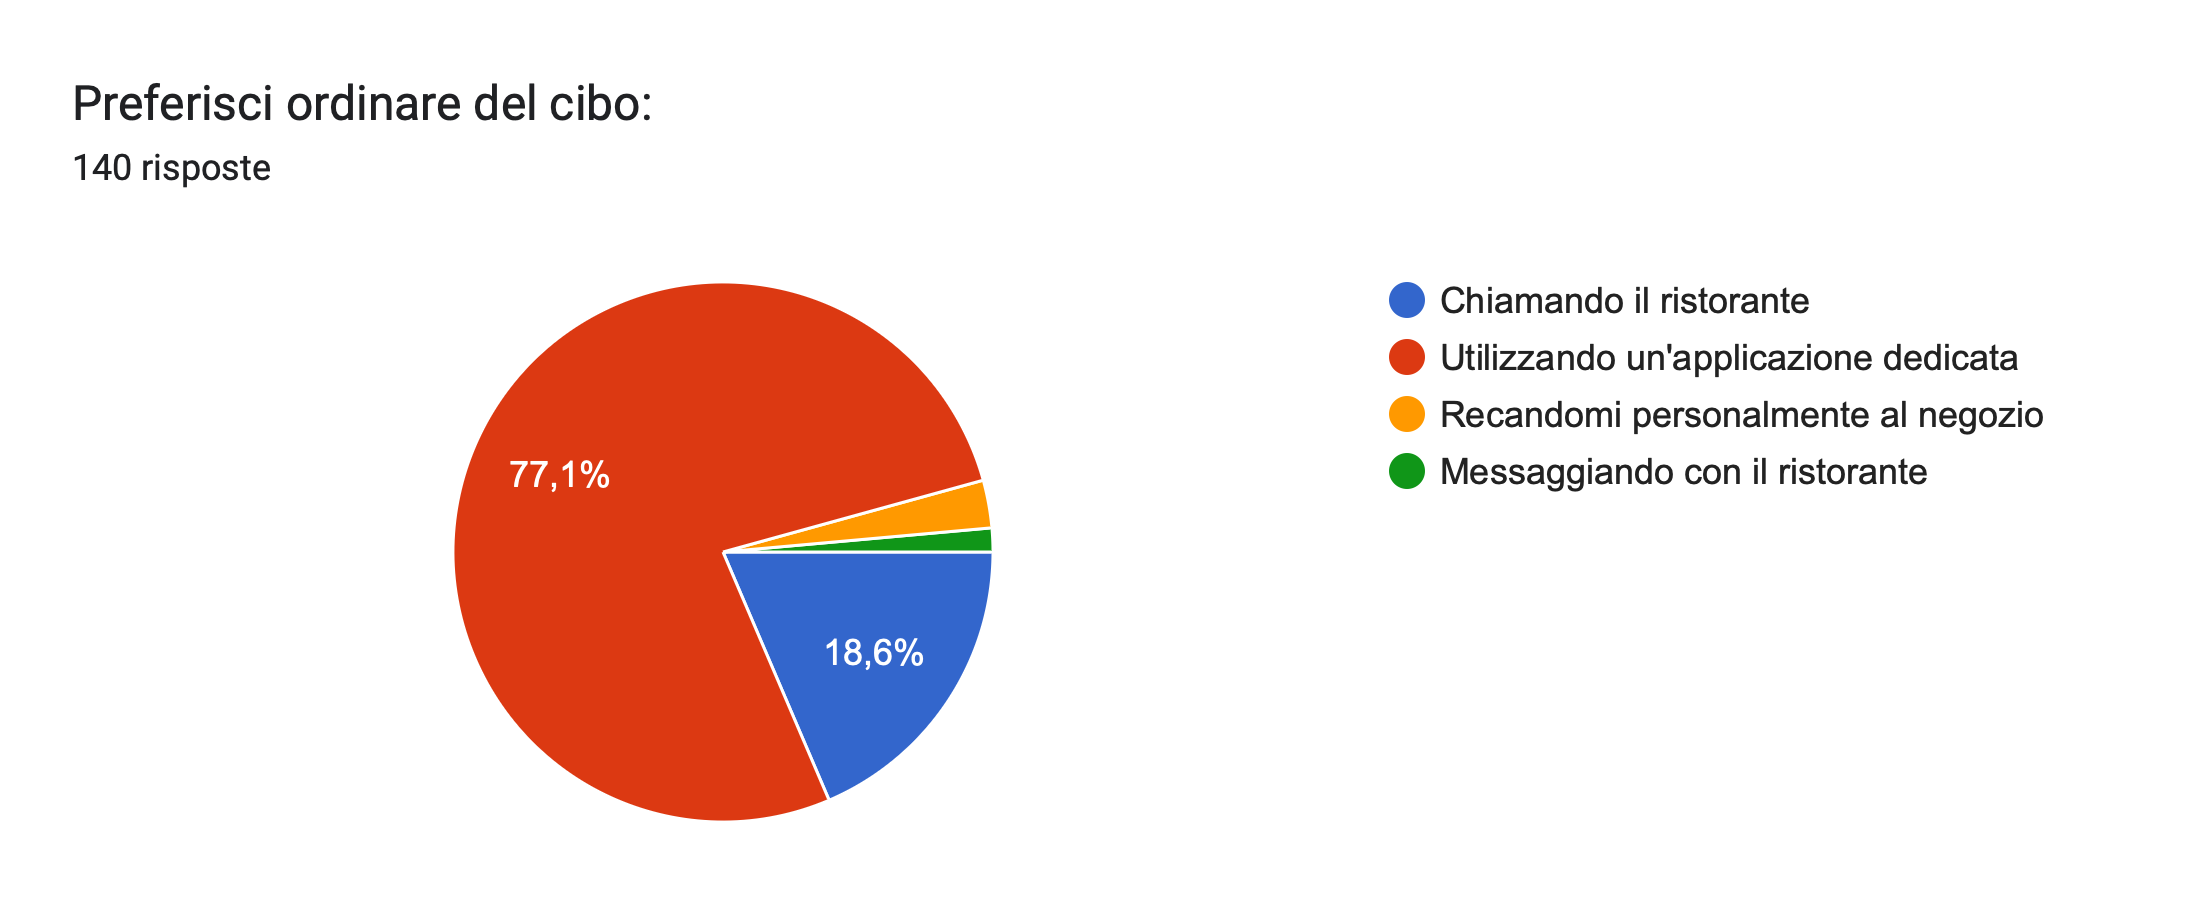
\includegraphics[width=\textwidth]{ordinare_cibo.png}\par
I nostri pensieri vengono confermati , perchè come possiamo notare una netta maggioranza preferisce ordinare cibo utilizzando un servizio dedicato, ben il 77,1\%.\par \vspace{1cm}
\includegraphics[width=\textwidth]{Funzionalità_fondamentali.png}\par
Dalle risposte ottenute individuiamo quali sono le funzionalità che saltano subito alla vista degli utenti:
\par \begin{itemize}
    \item Tracciamento dell'ordine;
    \item Abbinamenti cosigliati dal ristorante;
    \item Chattare con il rider;
    \item Visualizzare gli sconti disponibili;
\end{itemize}   \vspace{1cm} \par
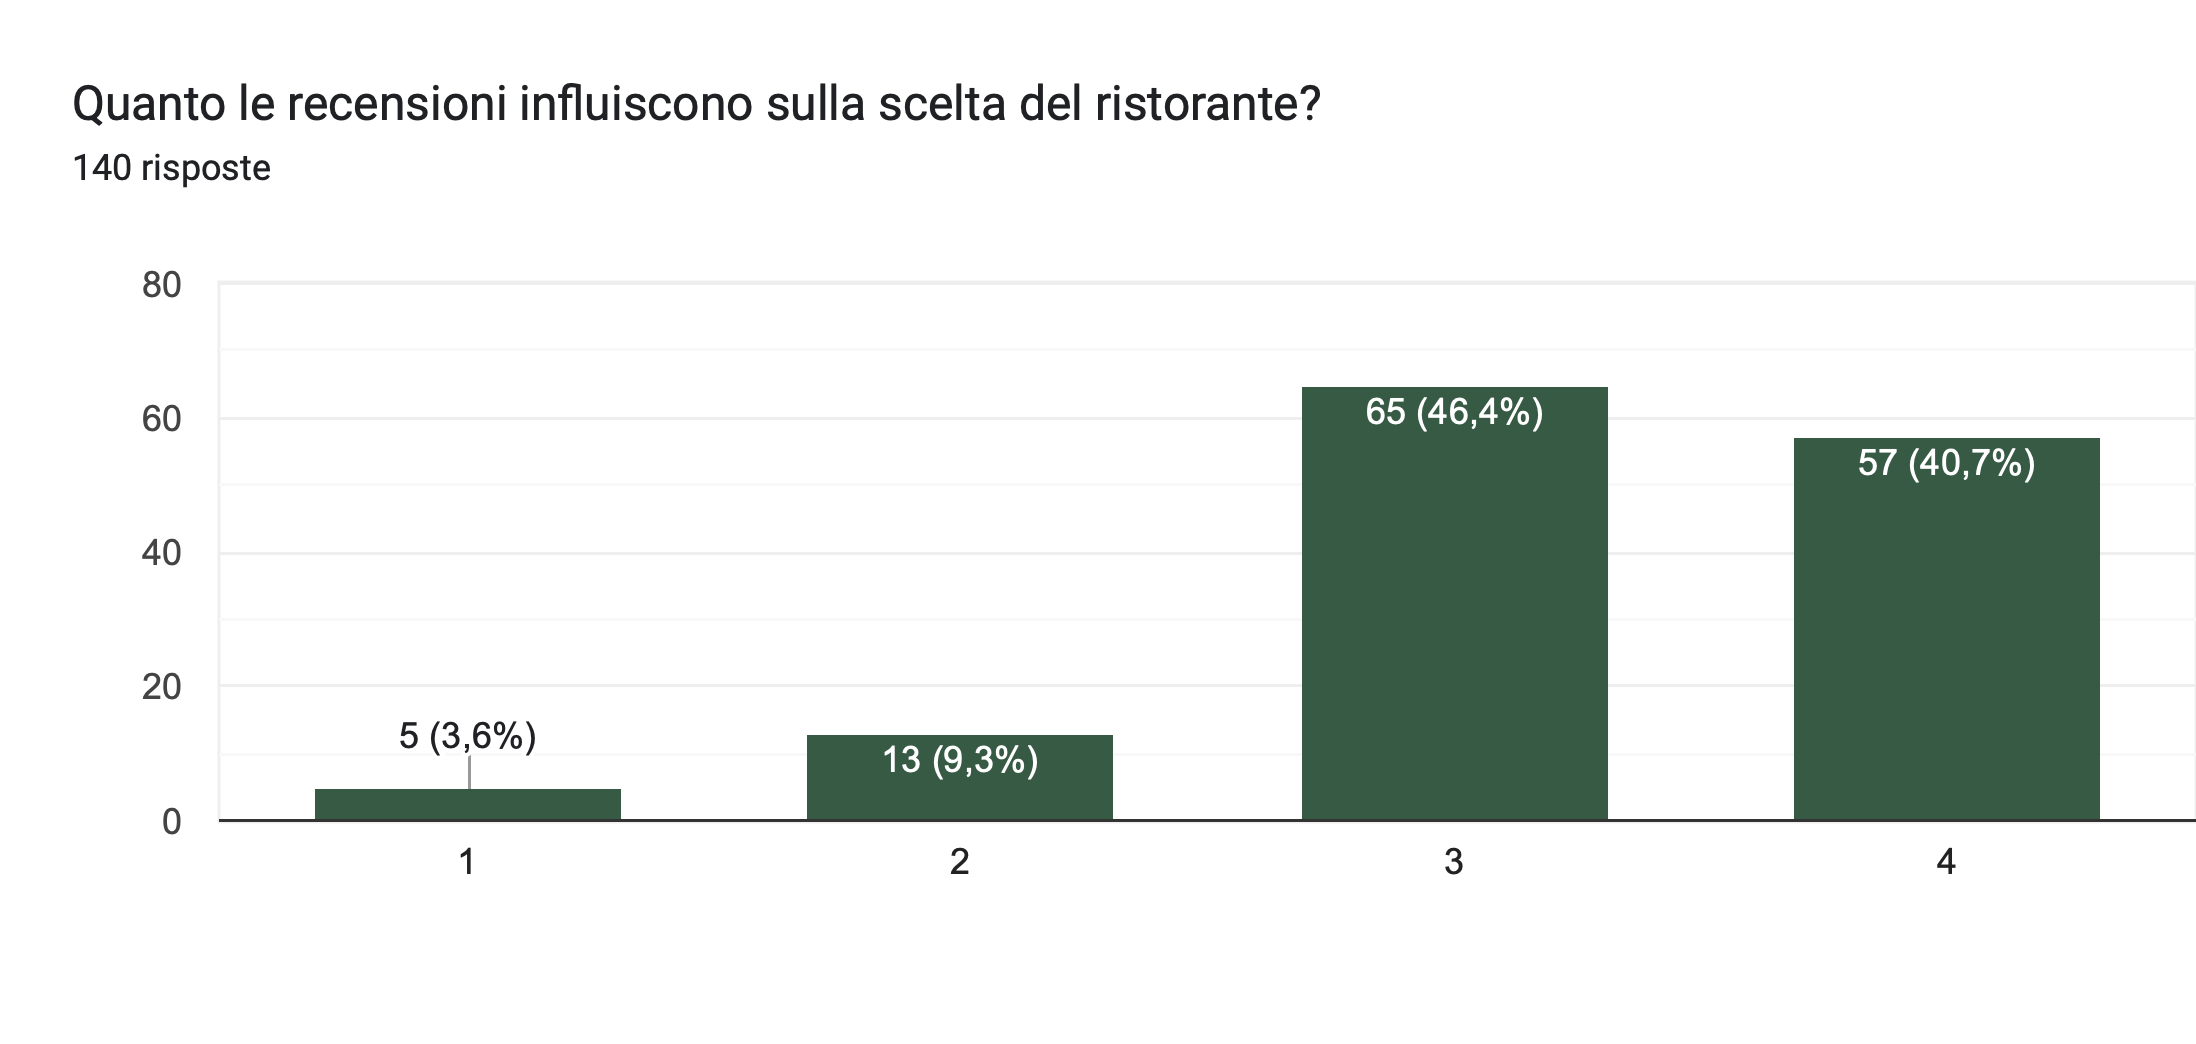
\includegraphics[width=\textwidth]{recensioni_influiscono.png}\par
Questa domanda è nata dall'idea di voler inserire una recensione 
    \begin{itemize}
        \item \textit{Per il ristorante}: di come gestisce l'ordine, se la cosegna viene effettuata in orario, e se il mantenimento del cibo e equo a quando si gusta nel ristorante.
        \item \textit{Per il piatto}: dare un voto al piatto che si ordina, se effettivamente rispetta le aspettative o se vengono completamente deluse.
    \end{itemize}
    \par \vspace{1cm}
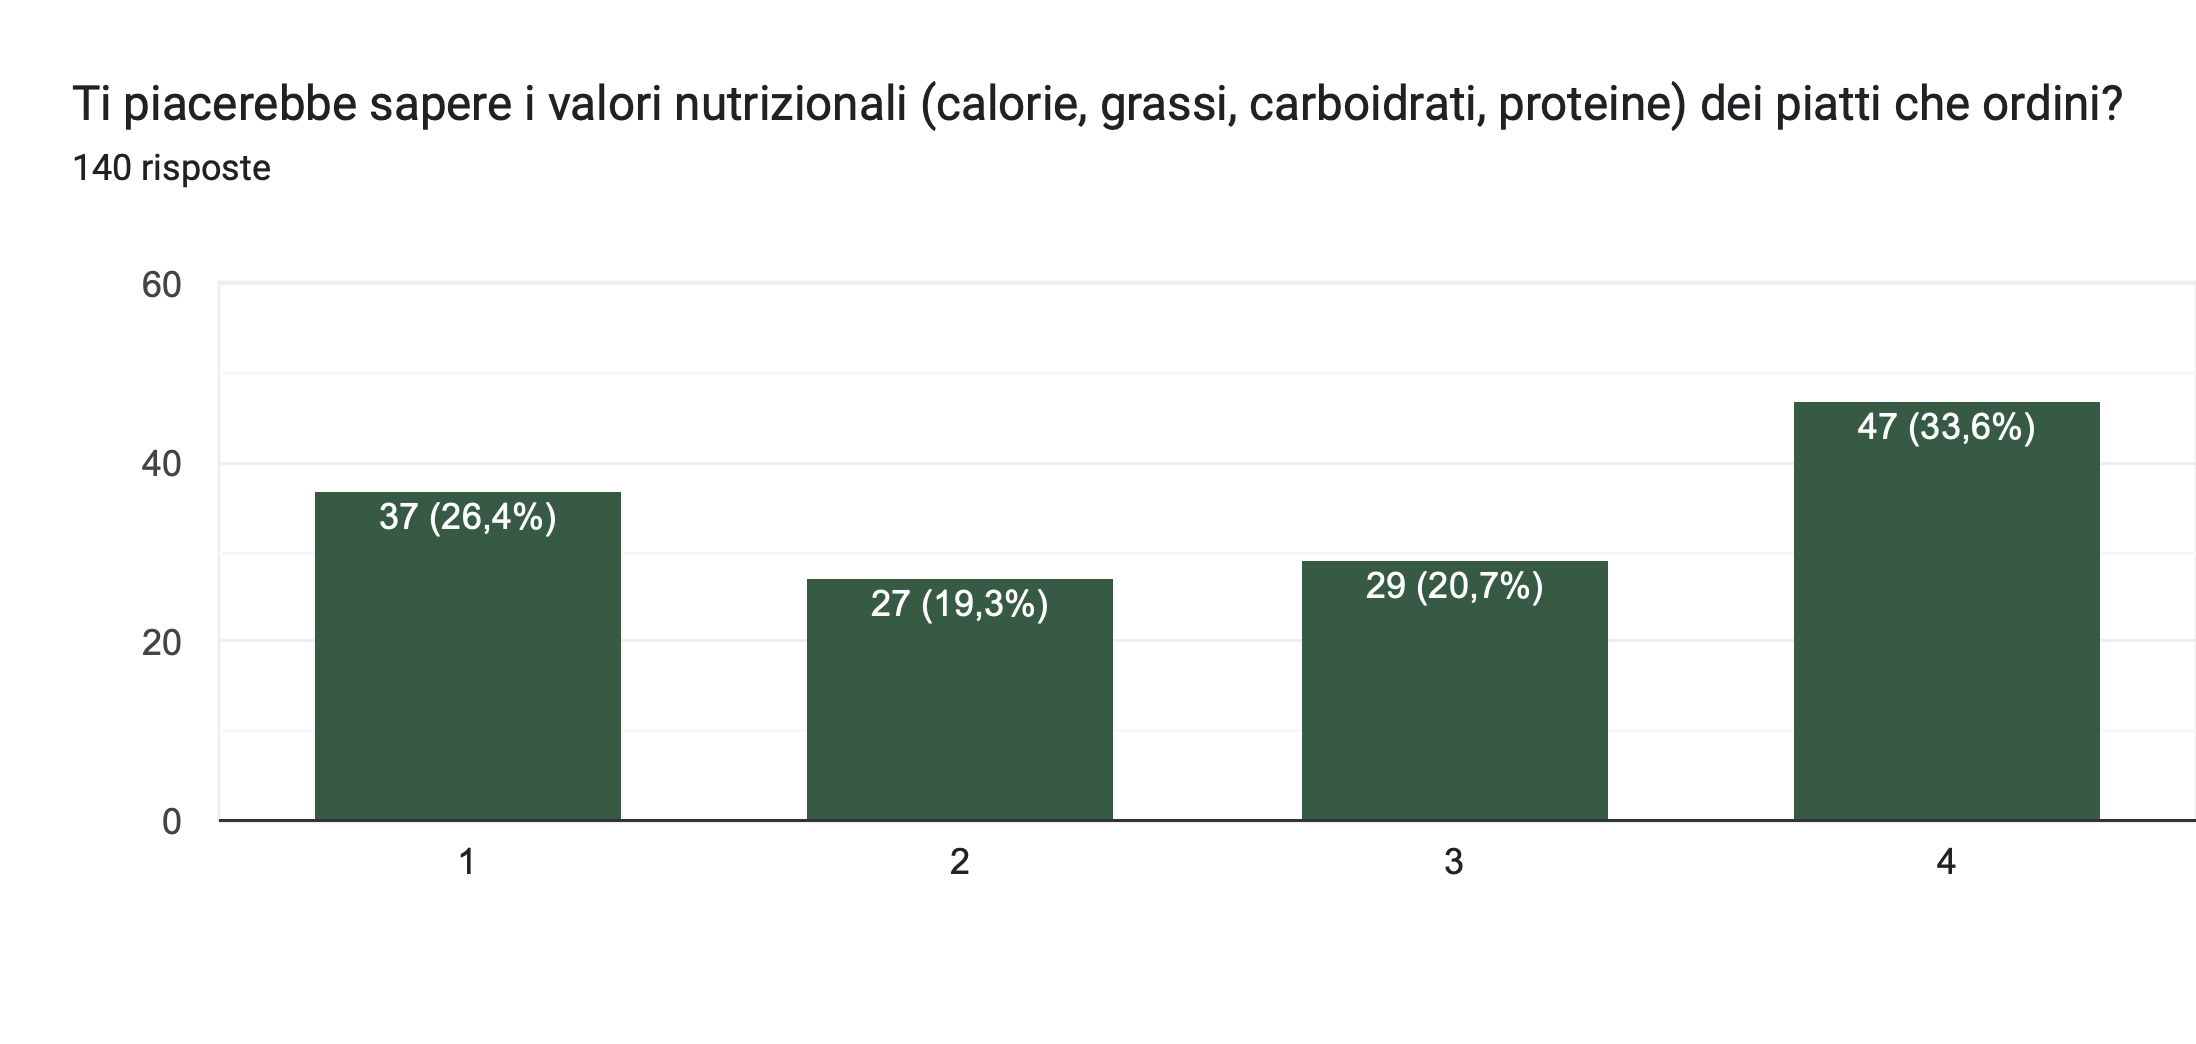
\includegraphics[width=\textwidth]{Valori_nutrizionali.png}\par
Per quanto le risposte di questa domanda, non possiamo dire che c'è una conferma definitiva, perchè i pareri sono abbasta differenti, nonostate la maggioranza, ovvero il 33,6\% lo preferiscono. \par
Inizialmente segnare i valori nutrizionali era un punto fondamentale del nostro servizio, ma a fine questionario e diventato più un punto secondario.\par \vspace{1cm}
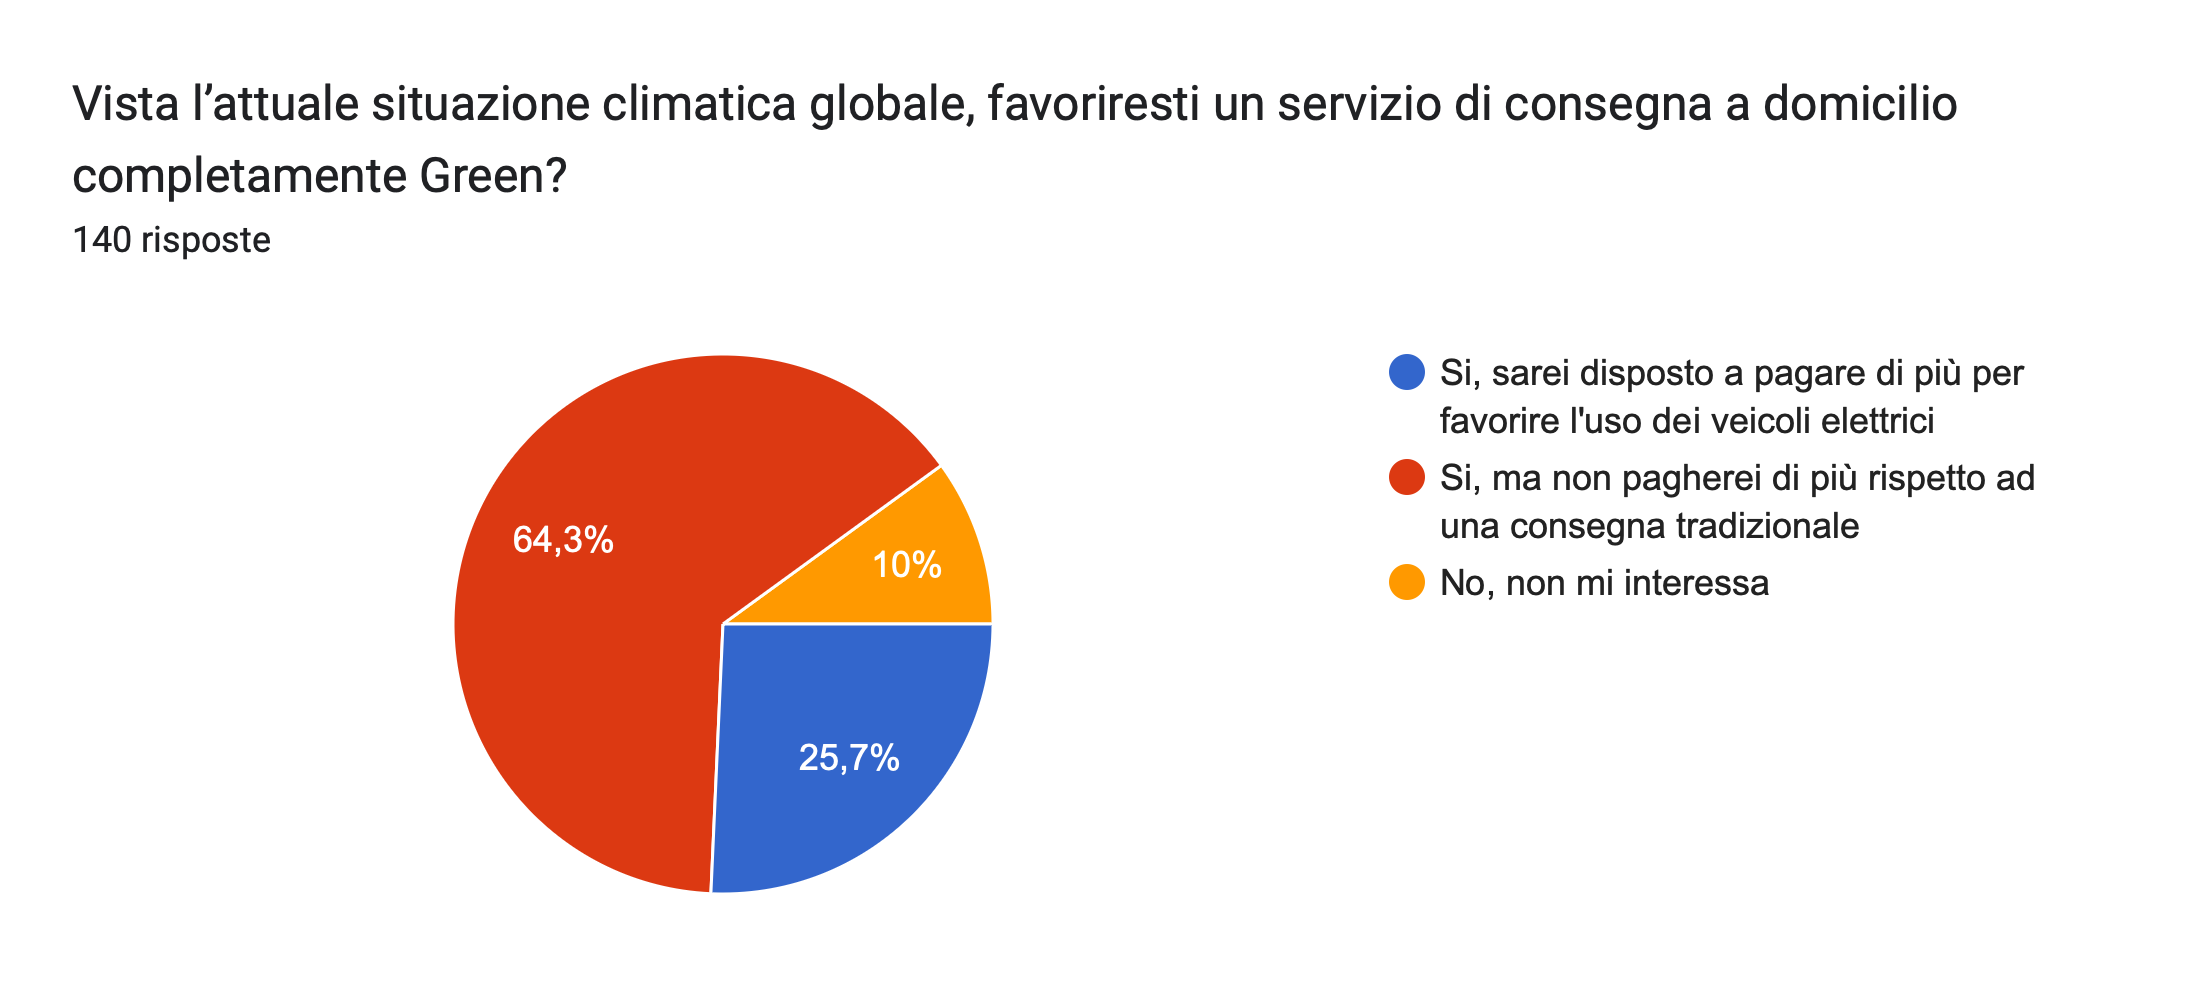
\includegraphics[width=\textwidth]{situazione_climatica.png}\par
Nonostante le interviste, in cui questa domanda ha creato più di un dibattito, nel questionario ne abbiamo la conferma, ovvero che a molti utenti interessa il salva-guardare ambientale, e l'orientamento verso un mondo sempre più eco-sostenibile.\par Notiamo che sommando le prime due risposte, si ha che ben il \textbf{90\%} userebbe il nostro servizio, ma ben il 64,3\% non sarebbe disposto ad un piccolo aumento di prezzo. \par \vspace{1cm}
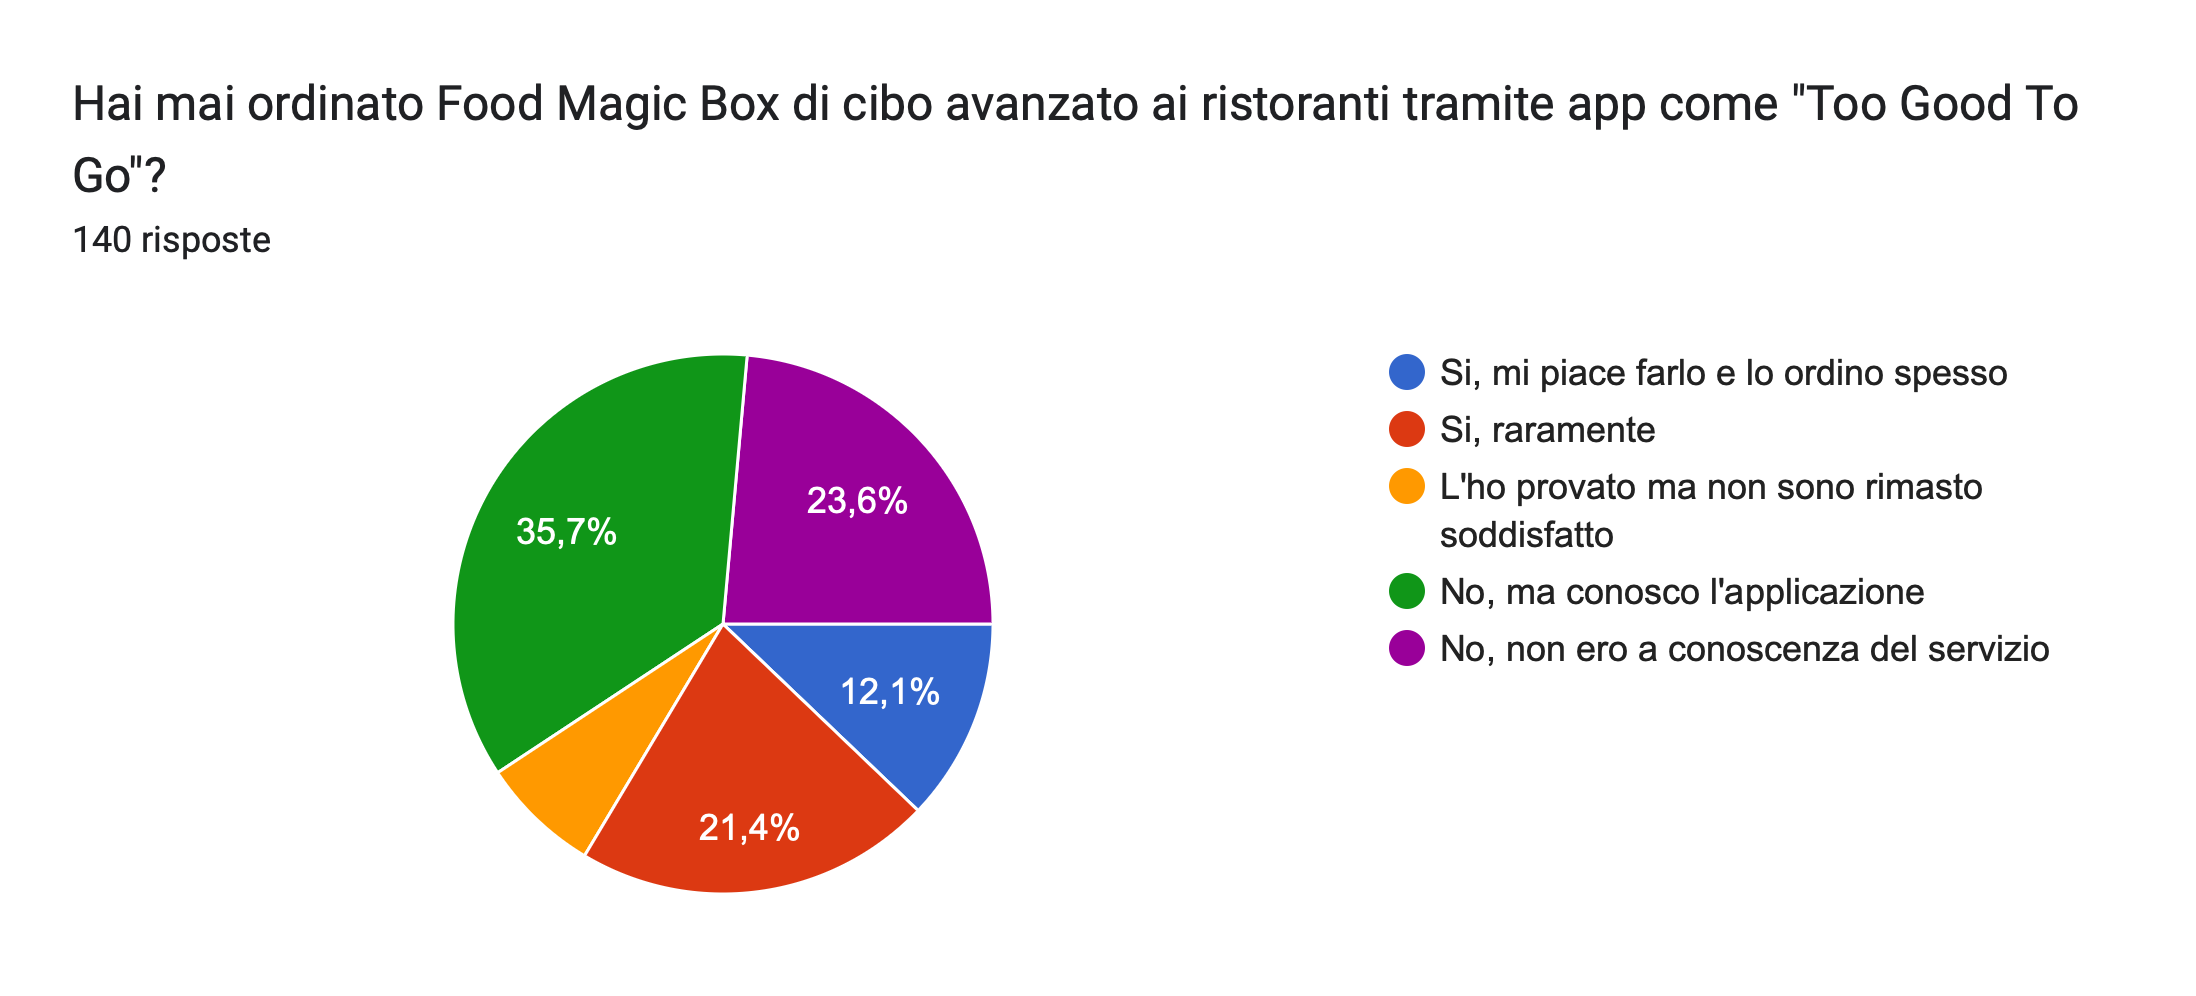
\includegraphics[width=\textwidth]{too_good_too_go.png}\par
Dalle risposte notiamo che solamente 33,5\& conosce e utilizza il servizio offerto da questa applicazione.\parVediamo che oltre il 35\% degli utenti che hanno risposto al questionario \textbf{non è a conoscenza} del servizio.\par \vspace{1cm}
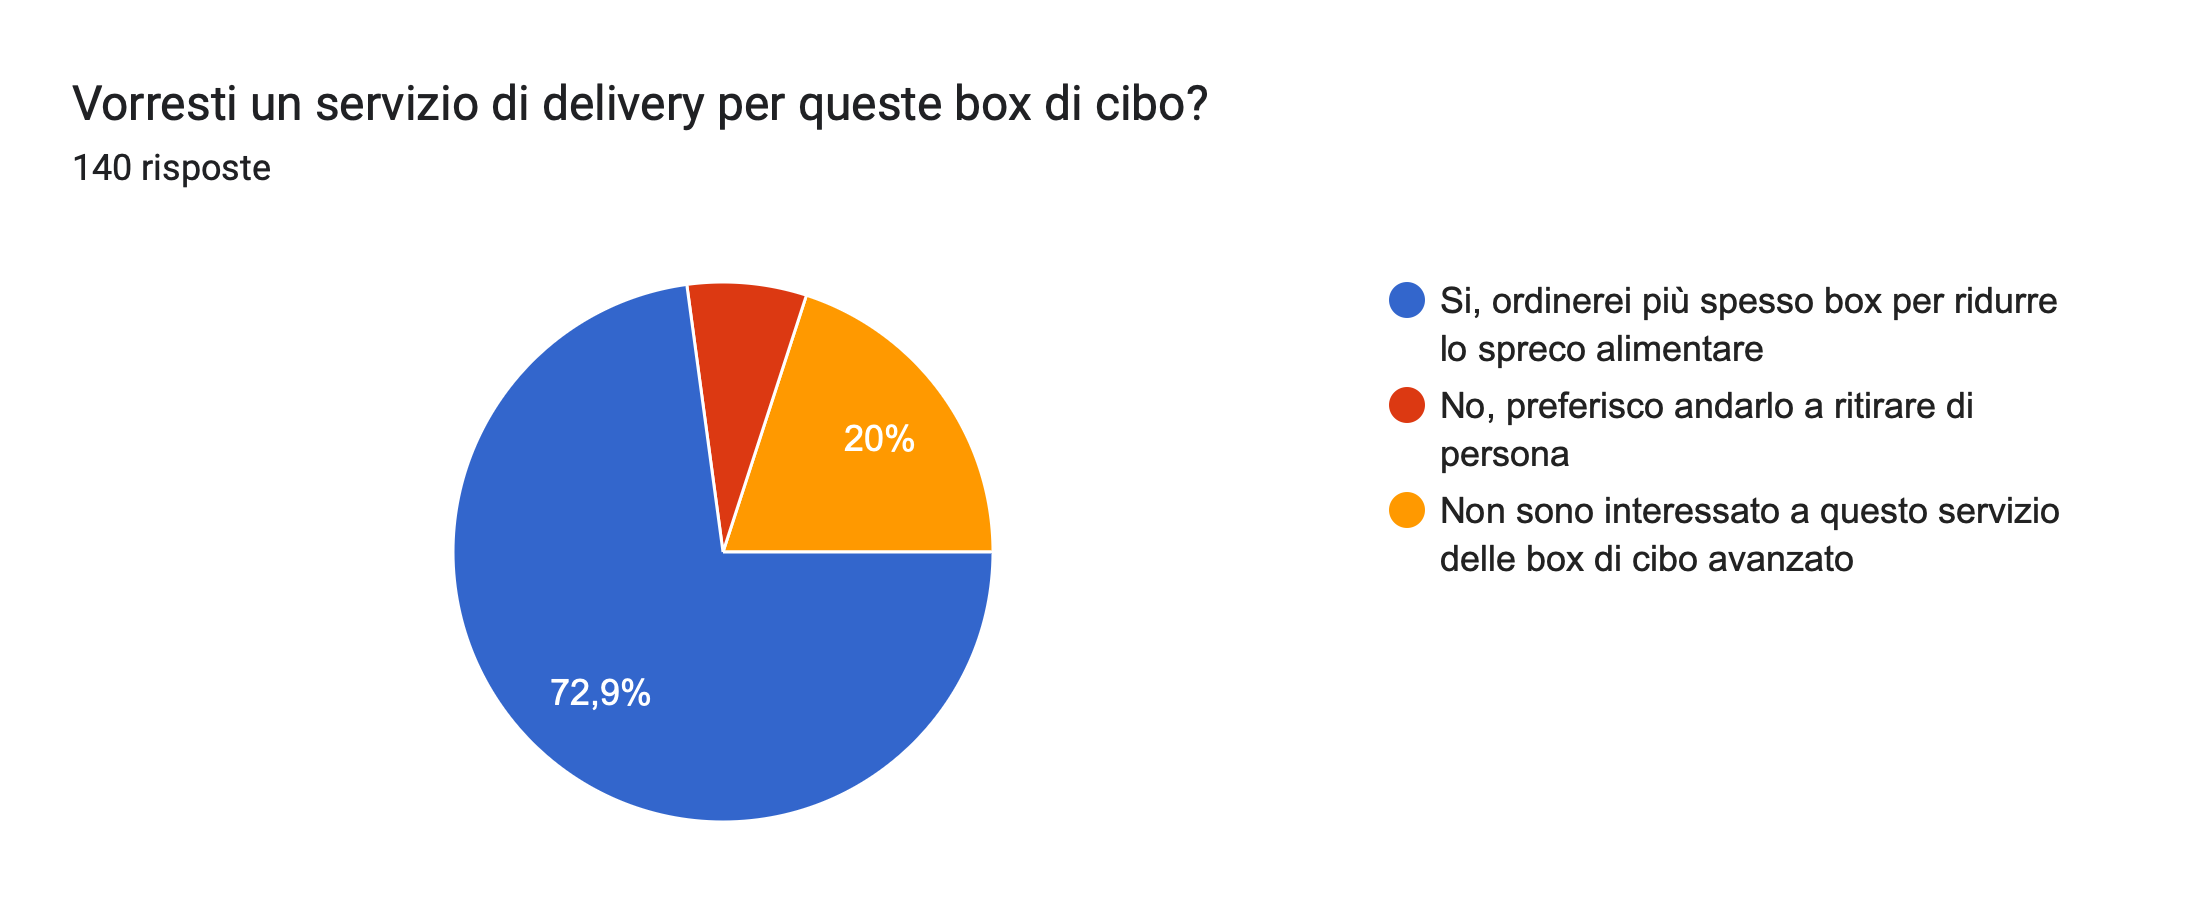
\includegraphics[width=\textwidth]{totg_delivery.png} \par
Abbiamo riscontrato che la maggior parte degli utenti(\textit{oltre 72\%}) sarebbe più propenso ad ordinare queste \textit{Magic-Box} se fossero ordinate a domicilio.
\begin{need}{}{theoexample}
    Dopo aver analizzato i risultati ottenuti dal questionario abbiamo riscontrato i seguenti need:
    \begin{enumerate}
        \item Risoluzione eventuali disguidi alla consegna.
        \item Combattere lo spreco alimentare.
        \item Visualizzazione su Maps dell'ordine mentre viene consegnato .
        \item Avere la possibilità di recensire sia il ristorante, sia la pietanza singola.
        \item Avere una sezione “preferiti” dei ristoranti.
        \item Poter pagare anche con paypal, o sempre in contanti.
        \item Avere a disposizione un \textit{segna-calorie} nel caso in cui si segua una dieta.
    \end{enumerate}
    \end{need}

    \vspace{1cm}




    \vspace{4cm}

\section{Storyboard} \par
Le seguenti storyboard illustrano le principali task che sono state individuate:
\vspace{1cm}
\addcontentsline{toc}{subsection}{\numberline{3.1} Effettuare un ordine }
\numberline{\fontsize{4mm}{1mm}\selectfont \textbf{3.1} \textbf{Effettuare un ordine}}
\begin{center}
    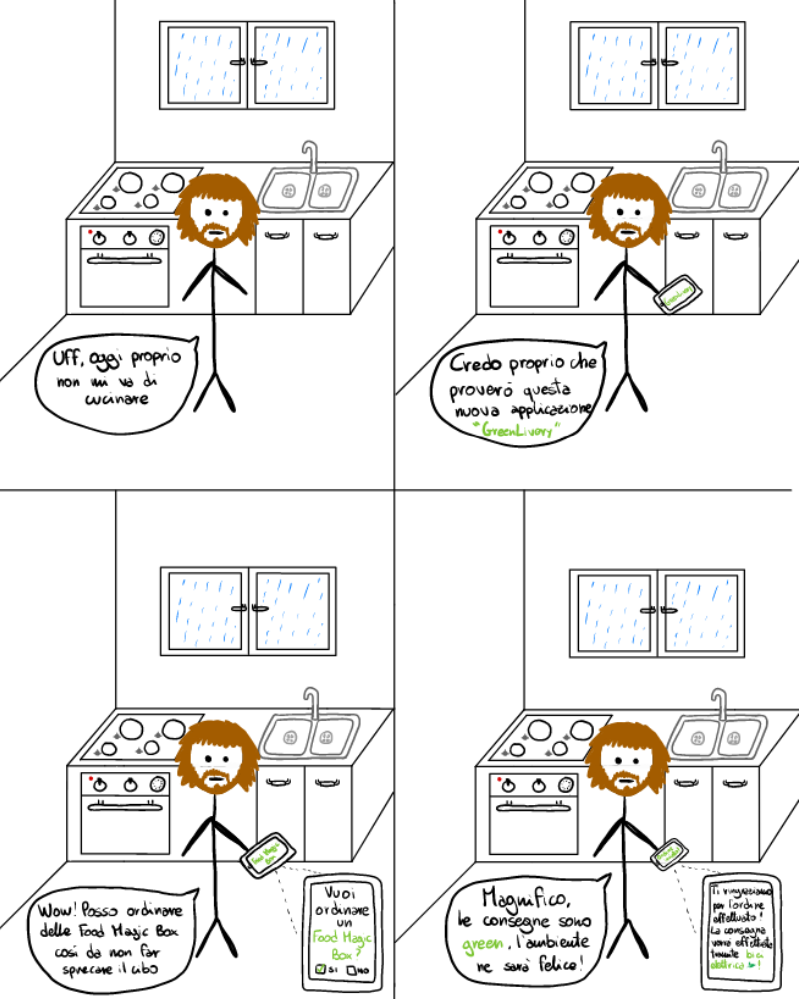
\includegraphics[scale=.3]{Effetuare_ordine.png}
\end{center}
\begin{itemize}
    \item \textbf{Descrizione scenario:}
    \item \textbf{Descrizione task:}
\end{itemize}
\addcontentsline{toc}{subsection}{\numberline{3.2} Usufruire dei servizi per avere una cosegna precisa}
\numberline{\fontsize{4mm}{1mm}\selectfont \textbf{3.2} Usufruire dei servizi per avere una cosegna precisa}
\begin{center}
    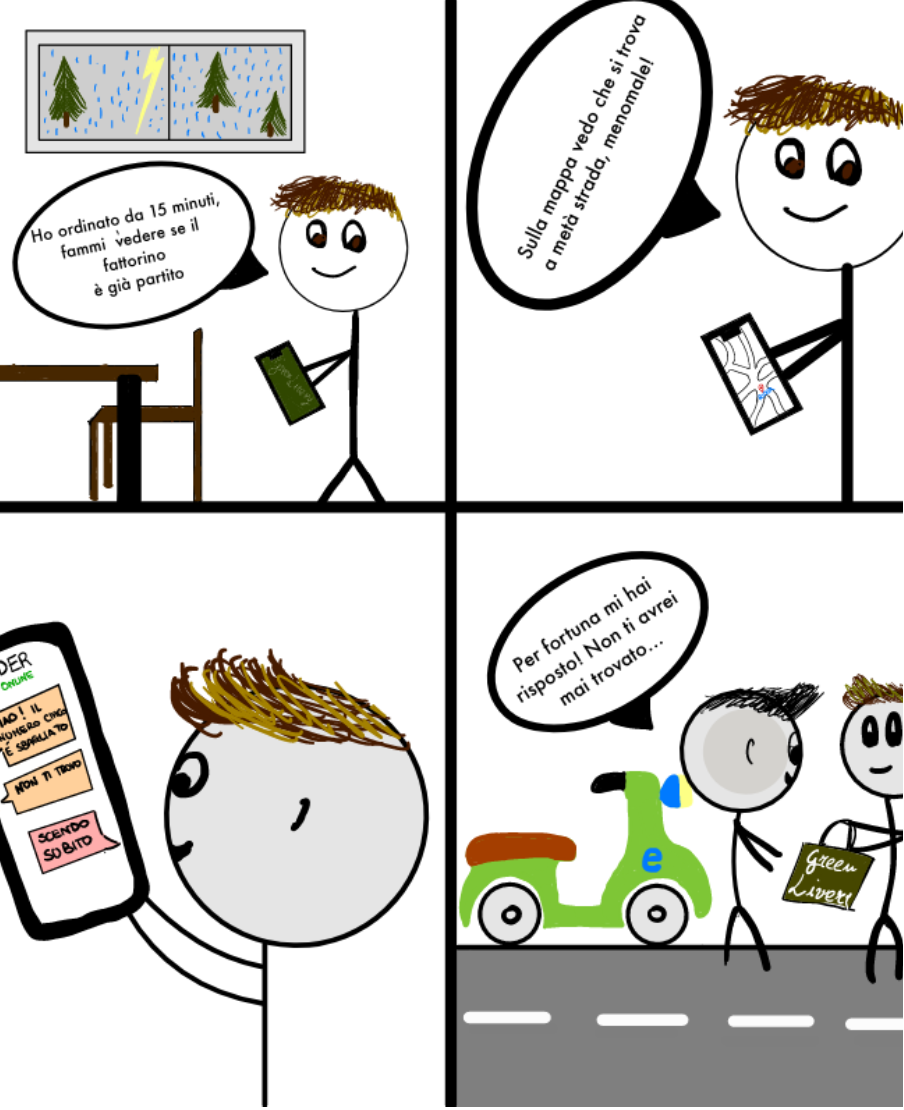
\includegraphics[scale=.3]{risoluzione disguidi alla cosegna.png}
\end{center}
\addcontentsline{toc}{subsection}{\numberline{3.3} Fornire valutazione ristorante e pietanza}
\numberline{\fontsize{4mm}{1mm}\selectfont \textbf{3.3} \textbf{Fornire valutazione ristorante e pietanza}}

\begin{center}
    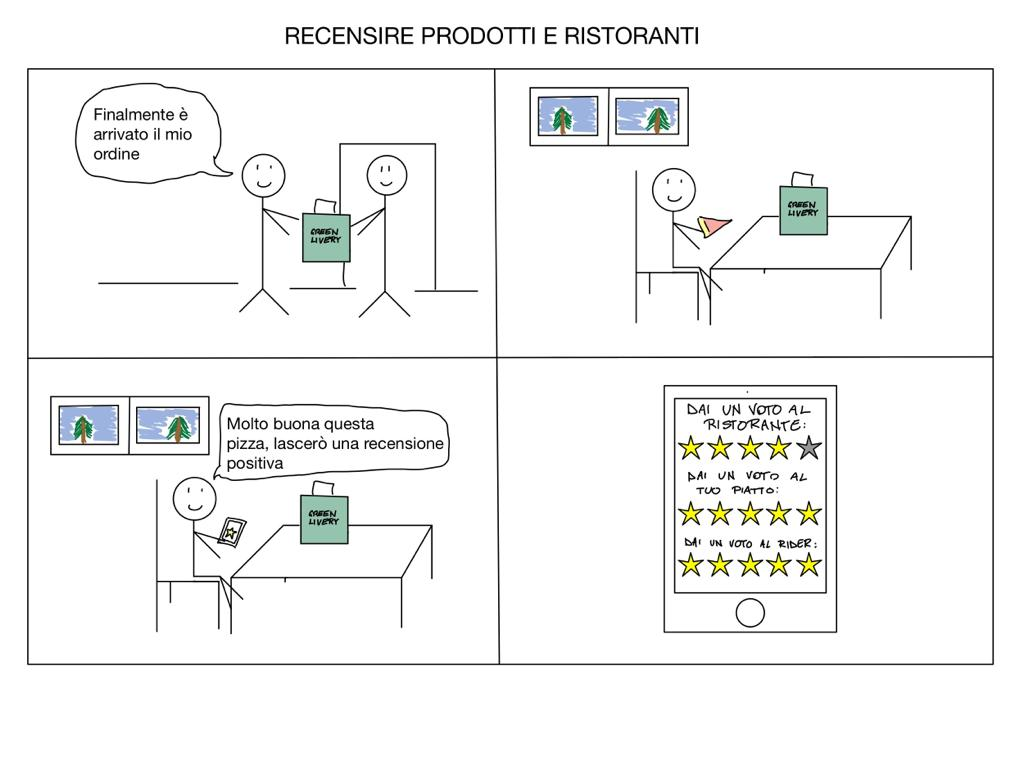
\includegraphics[scale=.3]{Recensioni.jpeg}
\end{center}

\begin{itemize}
    \item \textbf{Descrizione scenario:}
    \item \textbf{Descrizione task:}
\end{itemize}

\addcontentsline{toc}{subsection}{\numberline{3.4} Usufruire del segna-calorie se si segue una dieta}
\numberline{\fontsize{4mm}{1mm}\selectfont \textbf{3.4} \textbf{Usufruire del segna-calorie se si segue una dieta}}
\begin{center}
    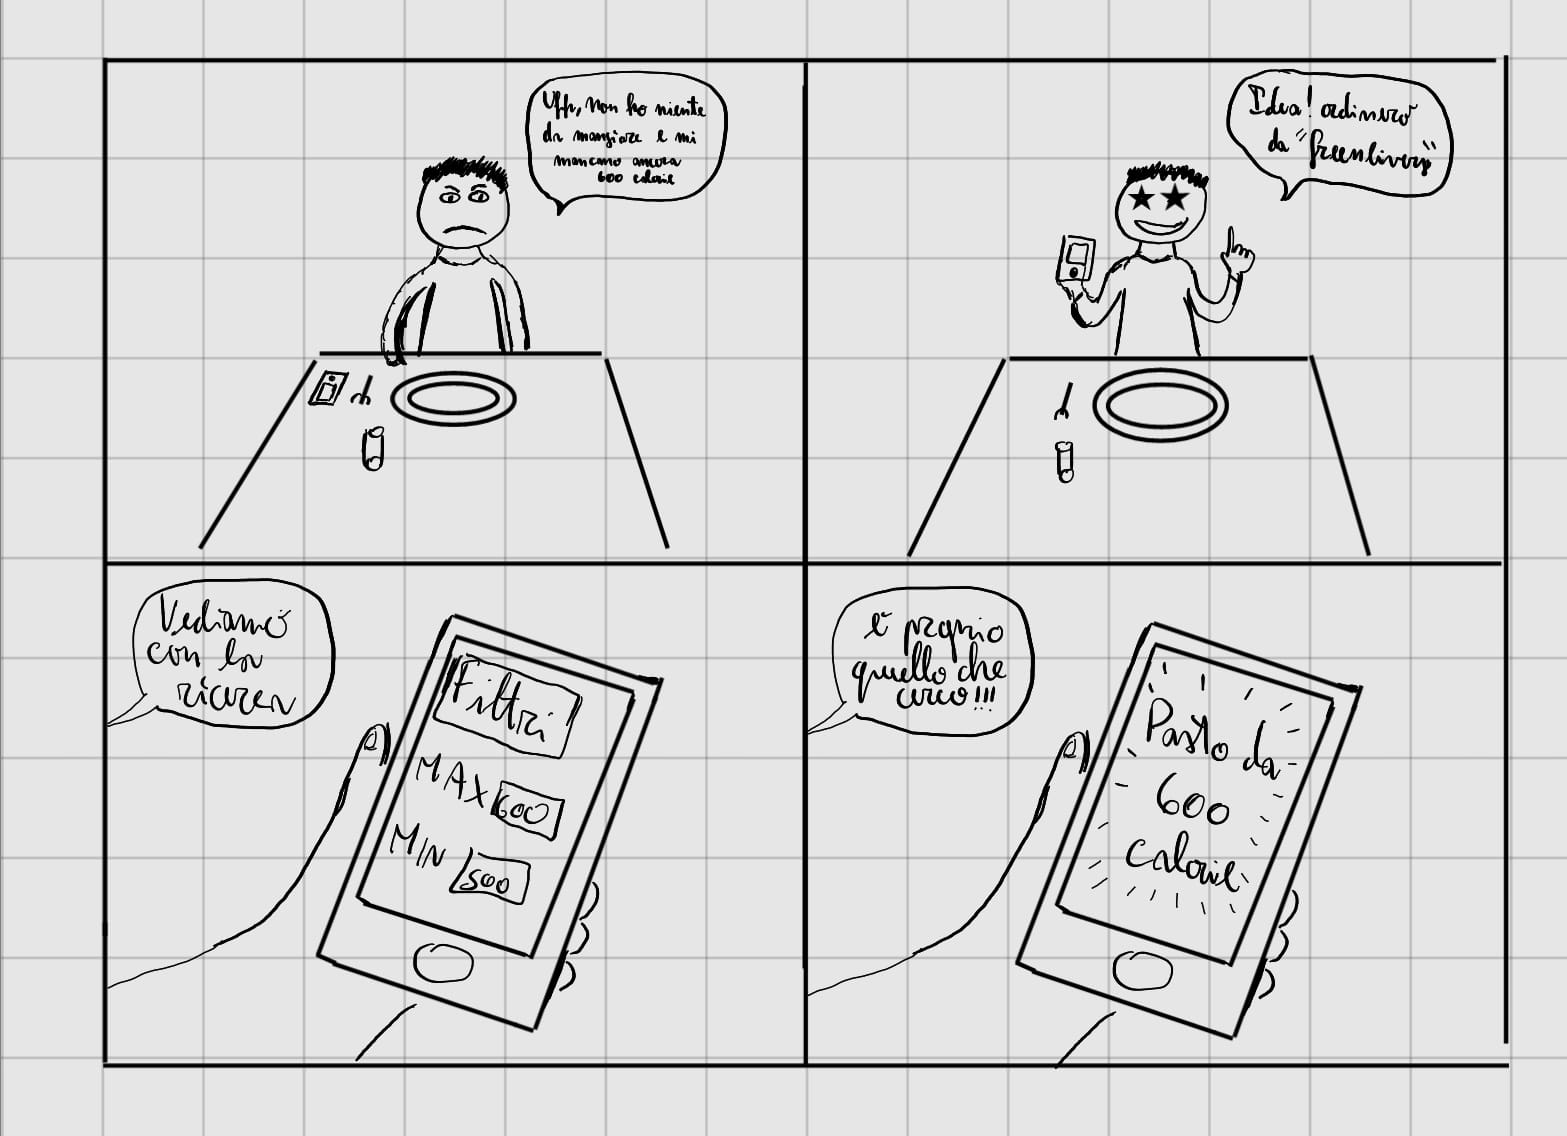
\includegraphics[scale=.3]{Filtro_calorie.jpeg}
\end{center}
\begin{itemize}
    \item \textbf{Descrizione scenario:}
    \item \textbf{Descrizione task:}
\end{itemize}

    
\section{Prototipi}

\vspace{1cm}
    \addcontentsline{toc}{subsection}{\numberline{4.1}Stile adoperato}             
    \numberline{\fontsize{4mm}{1mm}\selectfont \textbf{4.1 Stile adoperato}}
\par Lo stile adoperato\vspace{1cm}
    
    \addcontentsline{toc}{subsection}{\numberline{4.2}Funzionamento}               
    \numberline{\fontsize{4mm}{1mm}\selectfont \textbf{4.2 Funzionamento}}

    \vspace{1cm}
    
    \addcontentsline{toc}{subsection}{\numberline{4.3}Prototyping}                 
    \numberline{\fontsize{4mm}{1mm}\selectfont \textbf{4.3 Prototyping}}

    \vspace{1cm}

\section{UserTest}

\vspace{1cm}
    \addcontentsline{toc}{subsection}{\numberline{5.1}Stile }                      
    \numberline{\fontsize{4mm}{1mm}\selectfont \textbf{5.1 Stile}}

    \vspace{1cm}
    
    \addcontentsline{toc}{subsection}{\numberline{5.2}Numero utenti }              
    \numberline{\fontsize{4mm}{1mm}\selectfont \textbf{5.2 Numero utenti}}

    \vspace{1cm}
    
    \addcontentsline{toc}{subsection}{\numberline{5.3}Analisi risultati }          
    \numberline{\fontsize{4mm}{1mm}\selectfont \textbf{5.3 Analisi risultati}}

    \vspace{1cm}
    
\section{Problemi riscontrati durante la realizzazione del progetto}

\vspace{1cm}


\section{Revisioni}

Prendendo singolarmente le due revisioni effettuate durante il corso abbiamo riscontrato che:
\begin{itemize}\item \textbf{Prima revisione:} A seguito della prima revisione, effettuata il 14 dicembre, abbiamo riscontrato le seguenti problematiche:
    \begin{enumerate}
        \item Alcuni storyboard non chiari, in particolare il terzo e il quarto,e nel secondo ci è stato detto a fronte della rivisione che non era gradito l'unione di due need nello stesso task.
    \end{enumerate}
    \item\textbf{Seconda revisione:}
\end{itemize}











\end{document}